\documentclass[12pt,a4paper]{article}
\usepackage{amsmath, amssymb} % Math Packages
\usepackage{geometry}
\usepackage[hidelinks]{hyperref} % Clickable links
\usepackage{graphicx, float} % Image Packages
\graphicspath{{/home/tyler/Obsidian Vaults/Notes/Config}} % Path to image folder
\geometry{margin=2cm}
\setlength{\parindent}{0pt} % No indentation
\usepackage[table]{xcolor}
\usepackage{tabularx}
\usepackage{array}
\usepackage[none]{hyphenat} % Disable Hypens splitting words across lines
\usepackage{gensymb} 
\usepackage[backend=biber,style=apa]{biblatex}
\addbibresource{references.bib}
\begin{document}
\begin{center}
\textbf{\LARGE ENG306\\[6pt]
Power Electronics}\\[10pt]
\textbf{\large Lab 2\\[4pt]
Baley Eccles - 652137\\
Tyler Robards - 651790}\\
\end{center}

\tableofcontents
\newpage
\section{Introduction}
NOTE: Mention We had issues with saving data from the scope
\section{Diode Rectifiers}
\subsection{Half-Wave Rectifier with Resistive Load}
\textit{Plot(using data saved from the oscilloscope) or insert screenshots or sketch by hand, 
waveforms for $v_s$, $v_o$, $i_o$ and $v_D$ using the same time-scale x axis (so that they can be
easily compared – including diode voltage), and discuss your observations briefly.}\\

\begin{figure}[H]
\centering
\includegraphics[width=.7\columnwidth]{Images/20250828_124935.jpg}
\caption{\(V_s\) (yellow), \(V_o\) (green) and \(I_o\) (orange) for a half-wave rectifier with resistive load \label{fig:figure1}}
\end{figure}

As expected this is a half wave rectifier, as seen in Figure \ref{fig:figure1}. When the input voltage is positive the output voltage is positive, when the input voltage is negative the output voltage is zero. This is because the diode is blocking the negative voltages. This is also true for the current wave form.\\

\textit{From your waveform measurements using oscilloscope, compare the dc output current 
and voltage against digital multimeter measurements and also against values determined by applying 
theoretical relationships for this rectifier. Present the different measurements and calculated 
values in table form, commenting on your observations.}\\

The DC voltage can be calculated as seen in the following
\begin{align*}
V_{DC} &= \frac{V_m}{\pi} \\
V_{DC} &= \frac{V_{rms}\cdot\sqrt{2}}{\pi} \\
V_{DC} &= \frac{20\cdot\sqrt{2}}{\pi} \\
V_{DC} &= 9.0V
\end{align*}
The DC current then can simply be calculated using Ohms Law:
\[I_{DC} = \frac{V_{DC}}{R} = \frac{9}{48} = 0.188A\]

\begin{table}[H]
\caption{Theory and measured DC voltage and current for half-wave rectifier \label{tab:table1}}
\centering
\begin{tabular}{|c|c|c|}
\hline
 & Measured & Theory\\
\hline
DC Voltage (V) & 9.6 & 9.0\\
\hline
DC Current (mA) & 157 & 188\\
\hline
\end{tabular}
\end{table}\\

\subsection{Full-Wave Rectifier with Resistive and Inductive Load}
\textit{Why was it necessary to measure the rectifier supply voltage waveform using the oscilloscope
probes on the second of the two secondary windings or using two probes and the maths function?
Describe what you think would happen if probes were still placed across the first winding (i.e.
between points 1 and 2 on the circuit).}\\

To isolate the ground, the oscilloscope probes have common grounds. If the probes were still connected across terminals 1 and 2 and another probe was connected to the load, then the grounds shared between the probes would be located at different spots, creating a short between the input and the load. Hence connecting the probe across terminals 3 and 4 allows us to create a new ground reference that is not effected by the rest of the circuit.\\

\textit{For the resistive load only set up, plot (using data saved from the oscilloscope) or insert screenshots
or sketch by hand, waveforms for $v_s$, $v_o$, $i_o$ using the same time-scale x axis, and discuss your
observations.}\\

\begin{figure}[H]
\centering
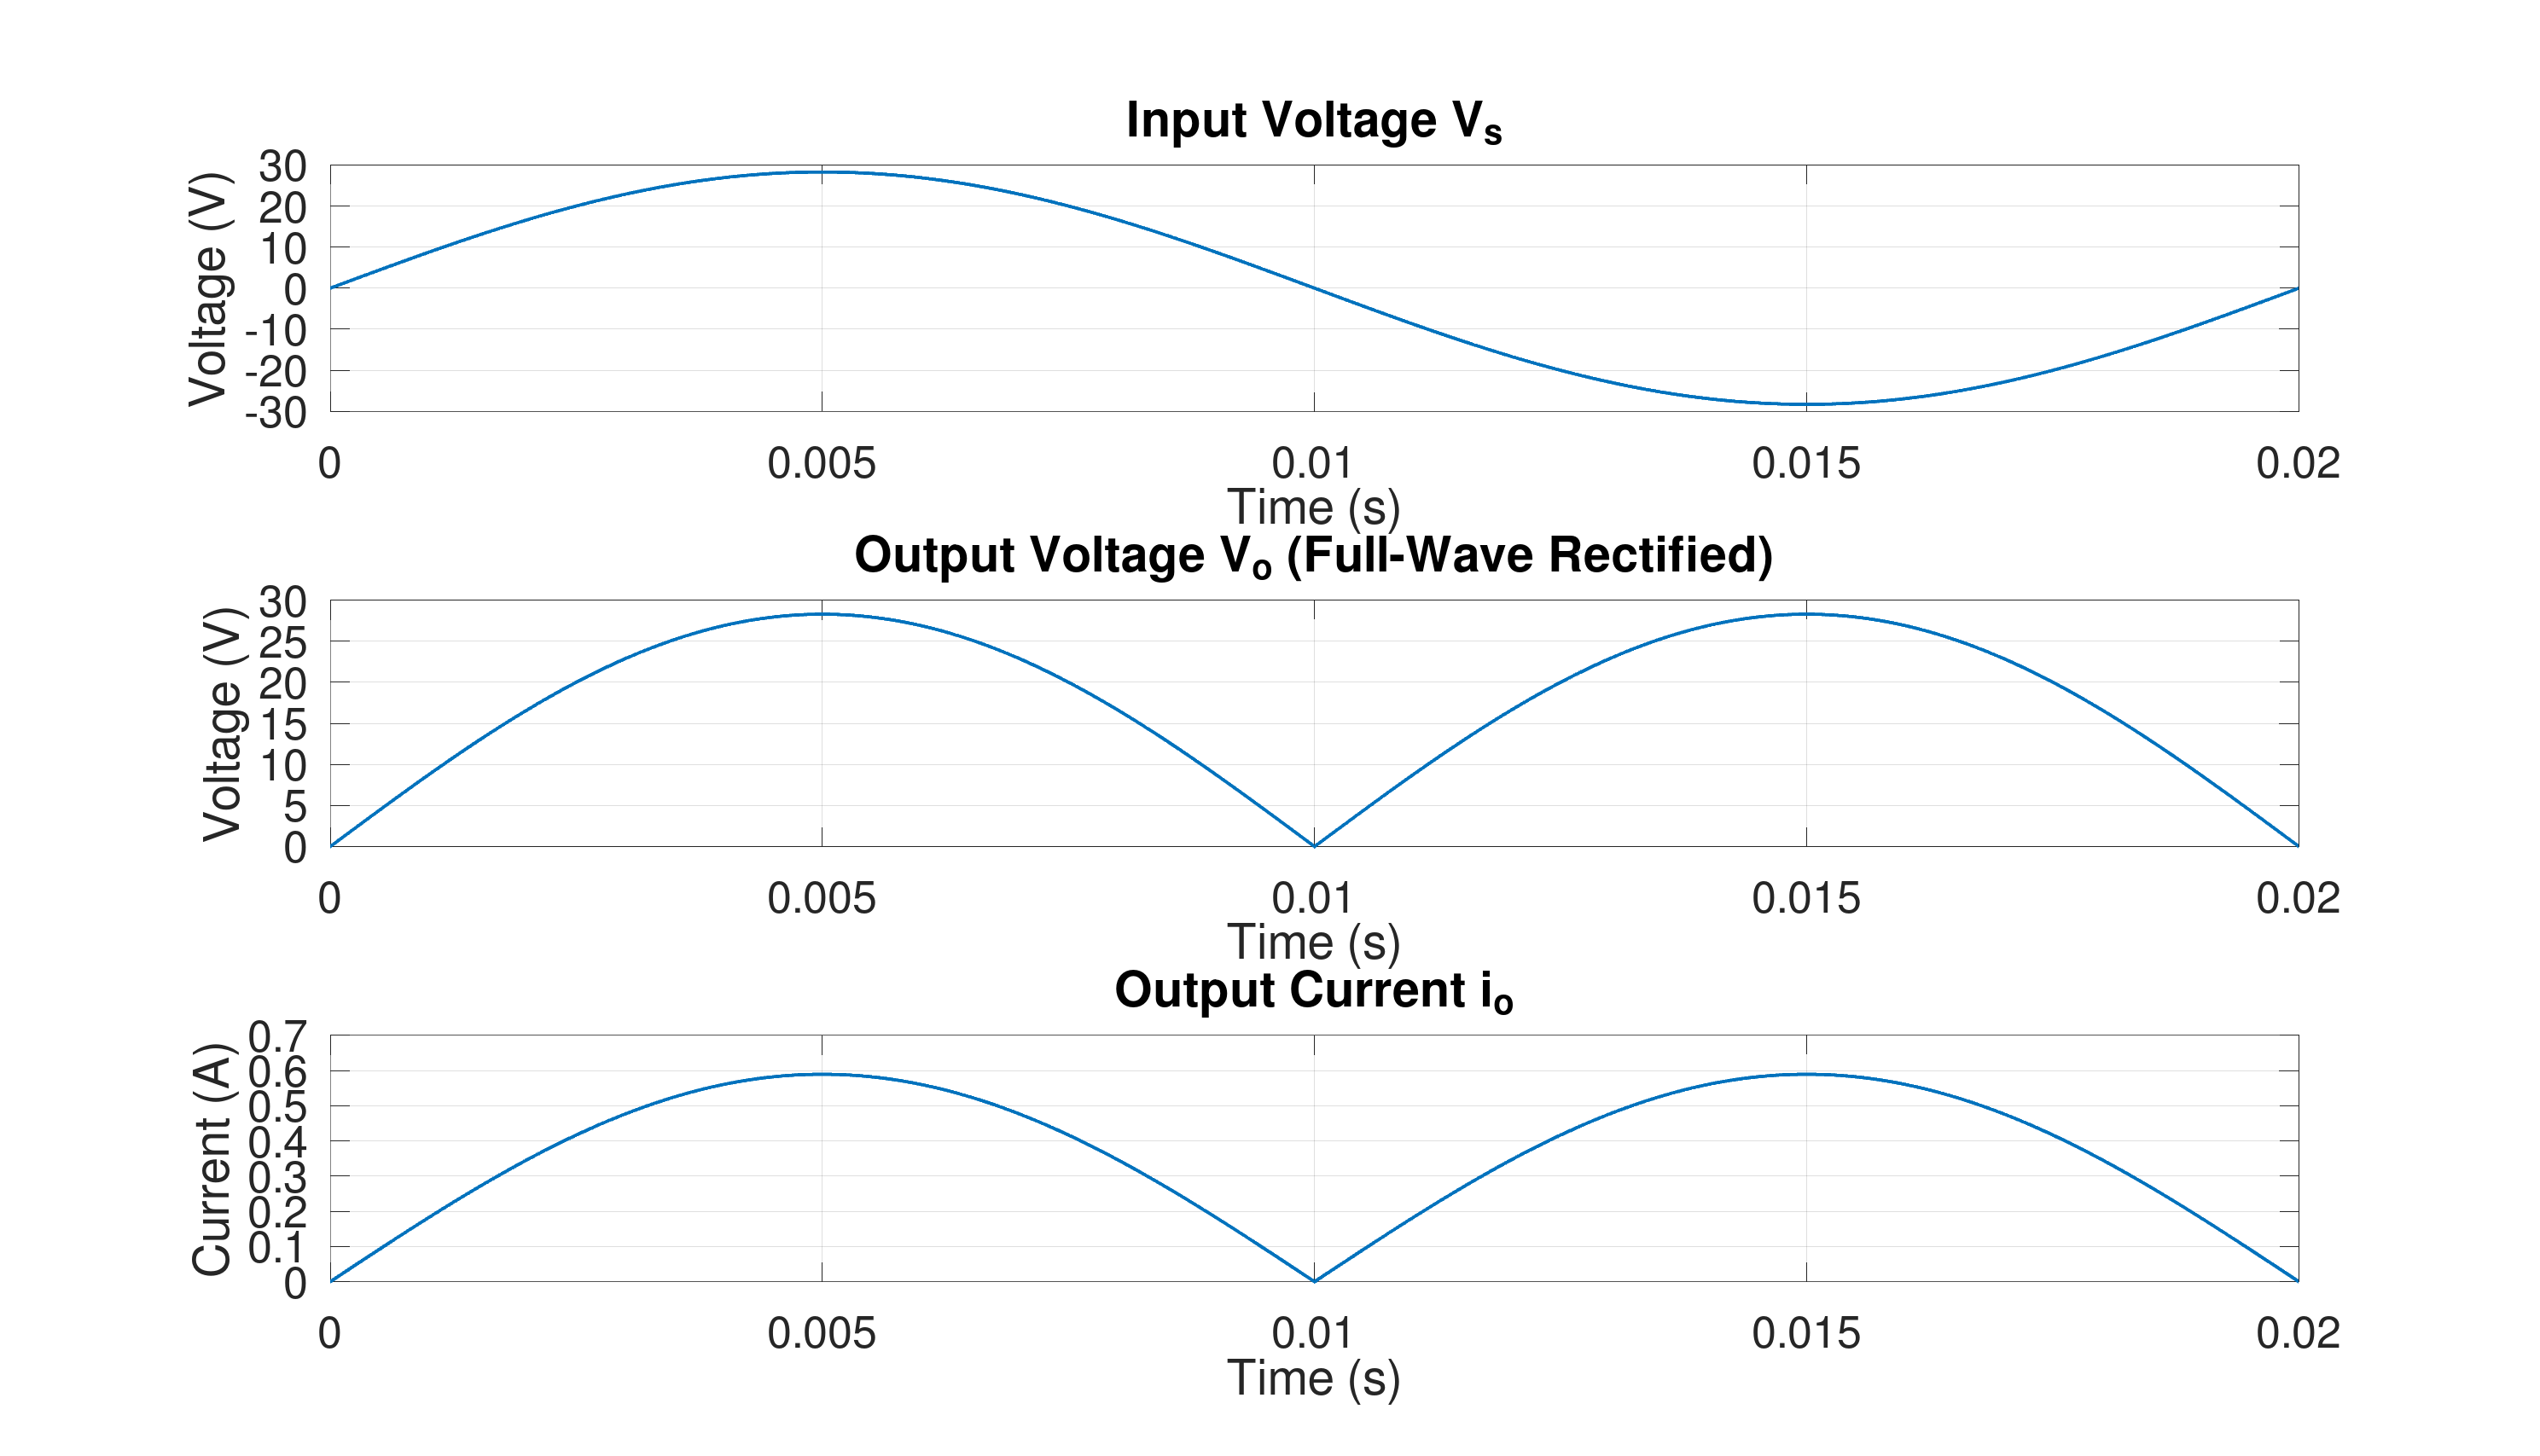
\includegraphics[width=.7\columnwidth]{ENG306_Lab_2_Full_Wave_Rectifier.png}
\caption{\(V_s\), \(V_o\) and \(I_o\) for a full-wave rectifier with resistive load \label{fig:figure2}}
\end{figure}

As expected the plot (Figure \ref{fig:figure2}) shows a full-wave rectified voltage, this was also seen in the lab, however a picture was not obtained. When the voltage is positive the two diodes $D_1$ and $D_2$ are forward biased and the other two diodes ($D_3$ and $D_4$) are reverse biased, and vise versa for negative voltages. This results in a full-wave rectified voltage and current.\\

\textit{Again for the resistive load only, from your waveform measurements using oscilloscope, compare
the DC output current and voltage against digital multimeter measurements and also against values
determined by applying theoretical relationships for this rectifier. Present the different measurements
and calculated values in table form, commenting on your observations.}\\

The DC voltage and current can be seen as in the following calculations:
\begin{align*}
V_{DC} &= \frac{2V_m}{\pi} \\
V_{DC} &= \frac{2V_{rms}\cdot\sqrt{2}}{\pi} \\
V_{DC} &= \frac{2 \cdot 20\cdot\sqrt{2}}{\pi} \\
V_{DC} &= 18.0V
\end{align*}
Then using Ohm's Law we can calculate the DC current
\[I_{DC} = \frac{V_{DC}}{R} = \frac{18}{48} = 0.375A\]

\begin{table}[H]
\caption{Theory and measured DC voltage and current for full-wave rectifier with purely resistive load \label{tab:table2}}
\centering
\begin{tabular}{|c|c|c|}
\hline
 & Measured & Theory\\
\hline
DC Voltage (V) & 16.2 & 18.0\\
\hline
DC Current (mA) & 338 & 375\\
\hline
\end{tabular}
\end{table}

Looking at Table \ref{tab:table2} it can be seen that the theoretical results are greater than the measured results, this is probably due to measurements and setup errors. However, it could also be due to not considering the losses in the diodes when calculating the voltage and current.\\

\textit{For the resistive and inductive load, plot (using data saved from the oscilloscope) or insert
screenshots or sketch by hand, waveforms for $v_s$, $v_o$, $i_o$ and $v_D$ for the two diodes measured, using
the same time-scale x axis (so that they can be easily compared – including diode voltage), and
discuss your observations, including comparing against what was observed for resistive only load}\\

\begin{figure}[H]
	\centering
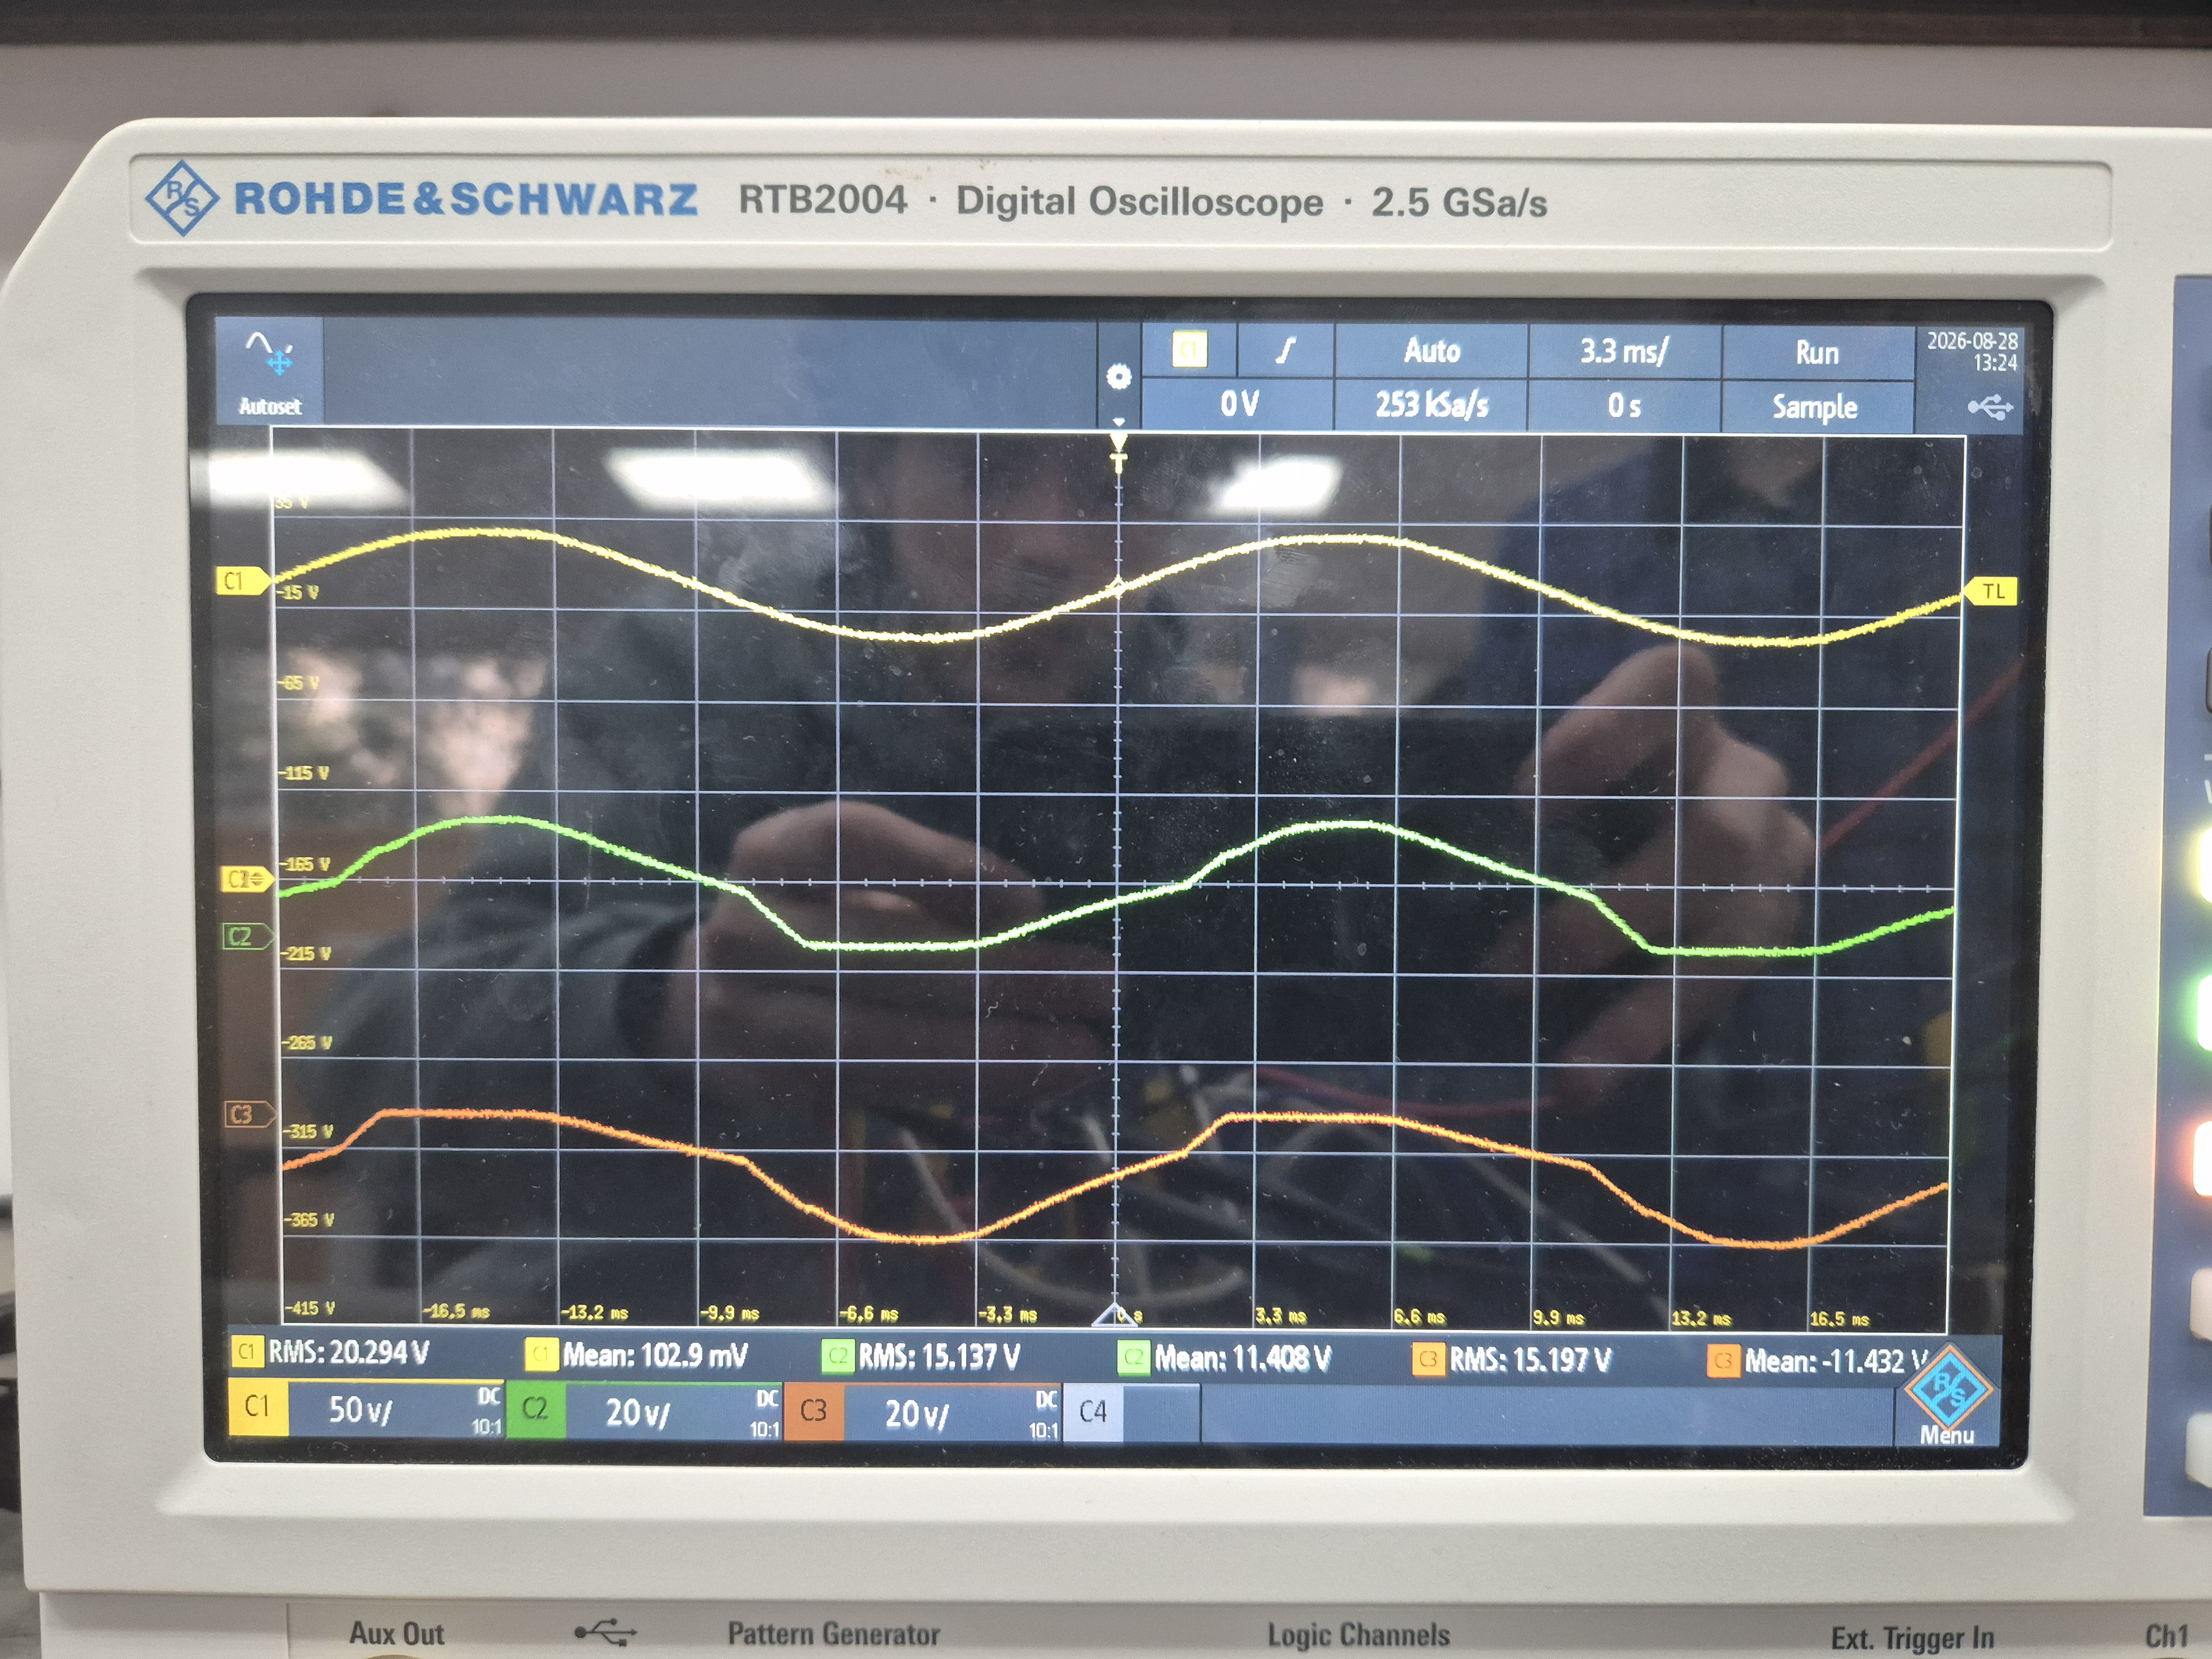
\includegraphics[width=.7\columnwidth]{Images/20250828_133520.jpg}
\caption{$V_s$, $V_o$ and $I_o$ for a full-wave rectifier with resistive and inductive load 
\label{fig:figure3}}
\end{figure}

The voltage across the load is a DC voltage with ripple, this can be seen in Figure \ref{fig:figure3}. This is because the inductor in the load stores energy (from current) and outputs current when the input current is negative. This results in the output voltage rising and reaching a steady state DC voltage with ripple.

The DC ripple for the inductive case is much less than the DC ripple in the purely resistive case. As mentioned this is because the inductor stores energy and releases it when necacary, creating a DC voltage.

\begin{figure}[H]
\centering
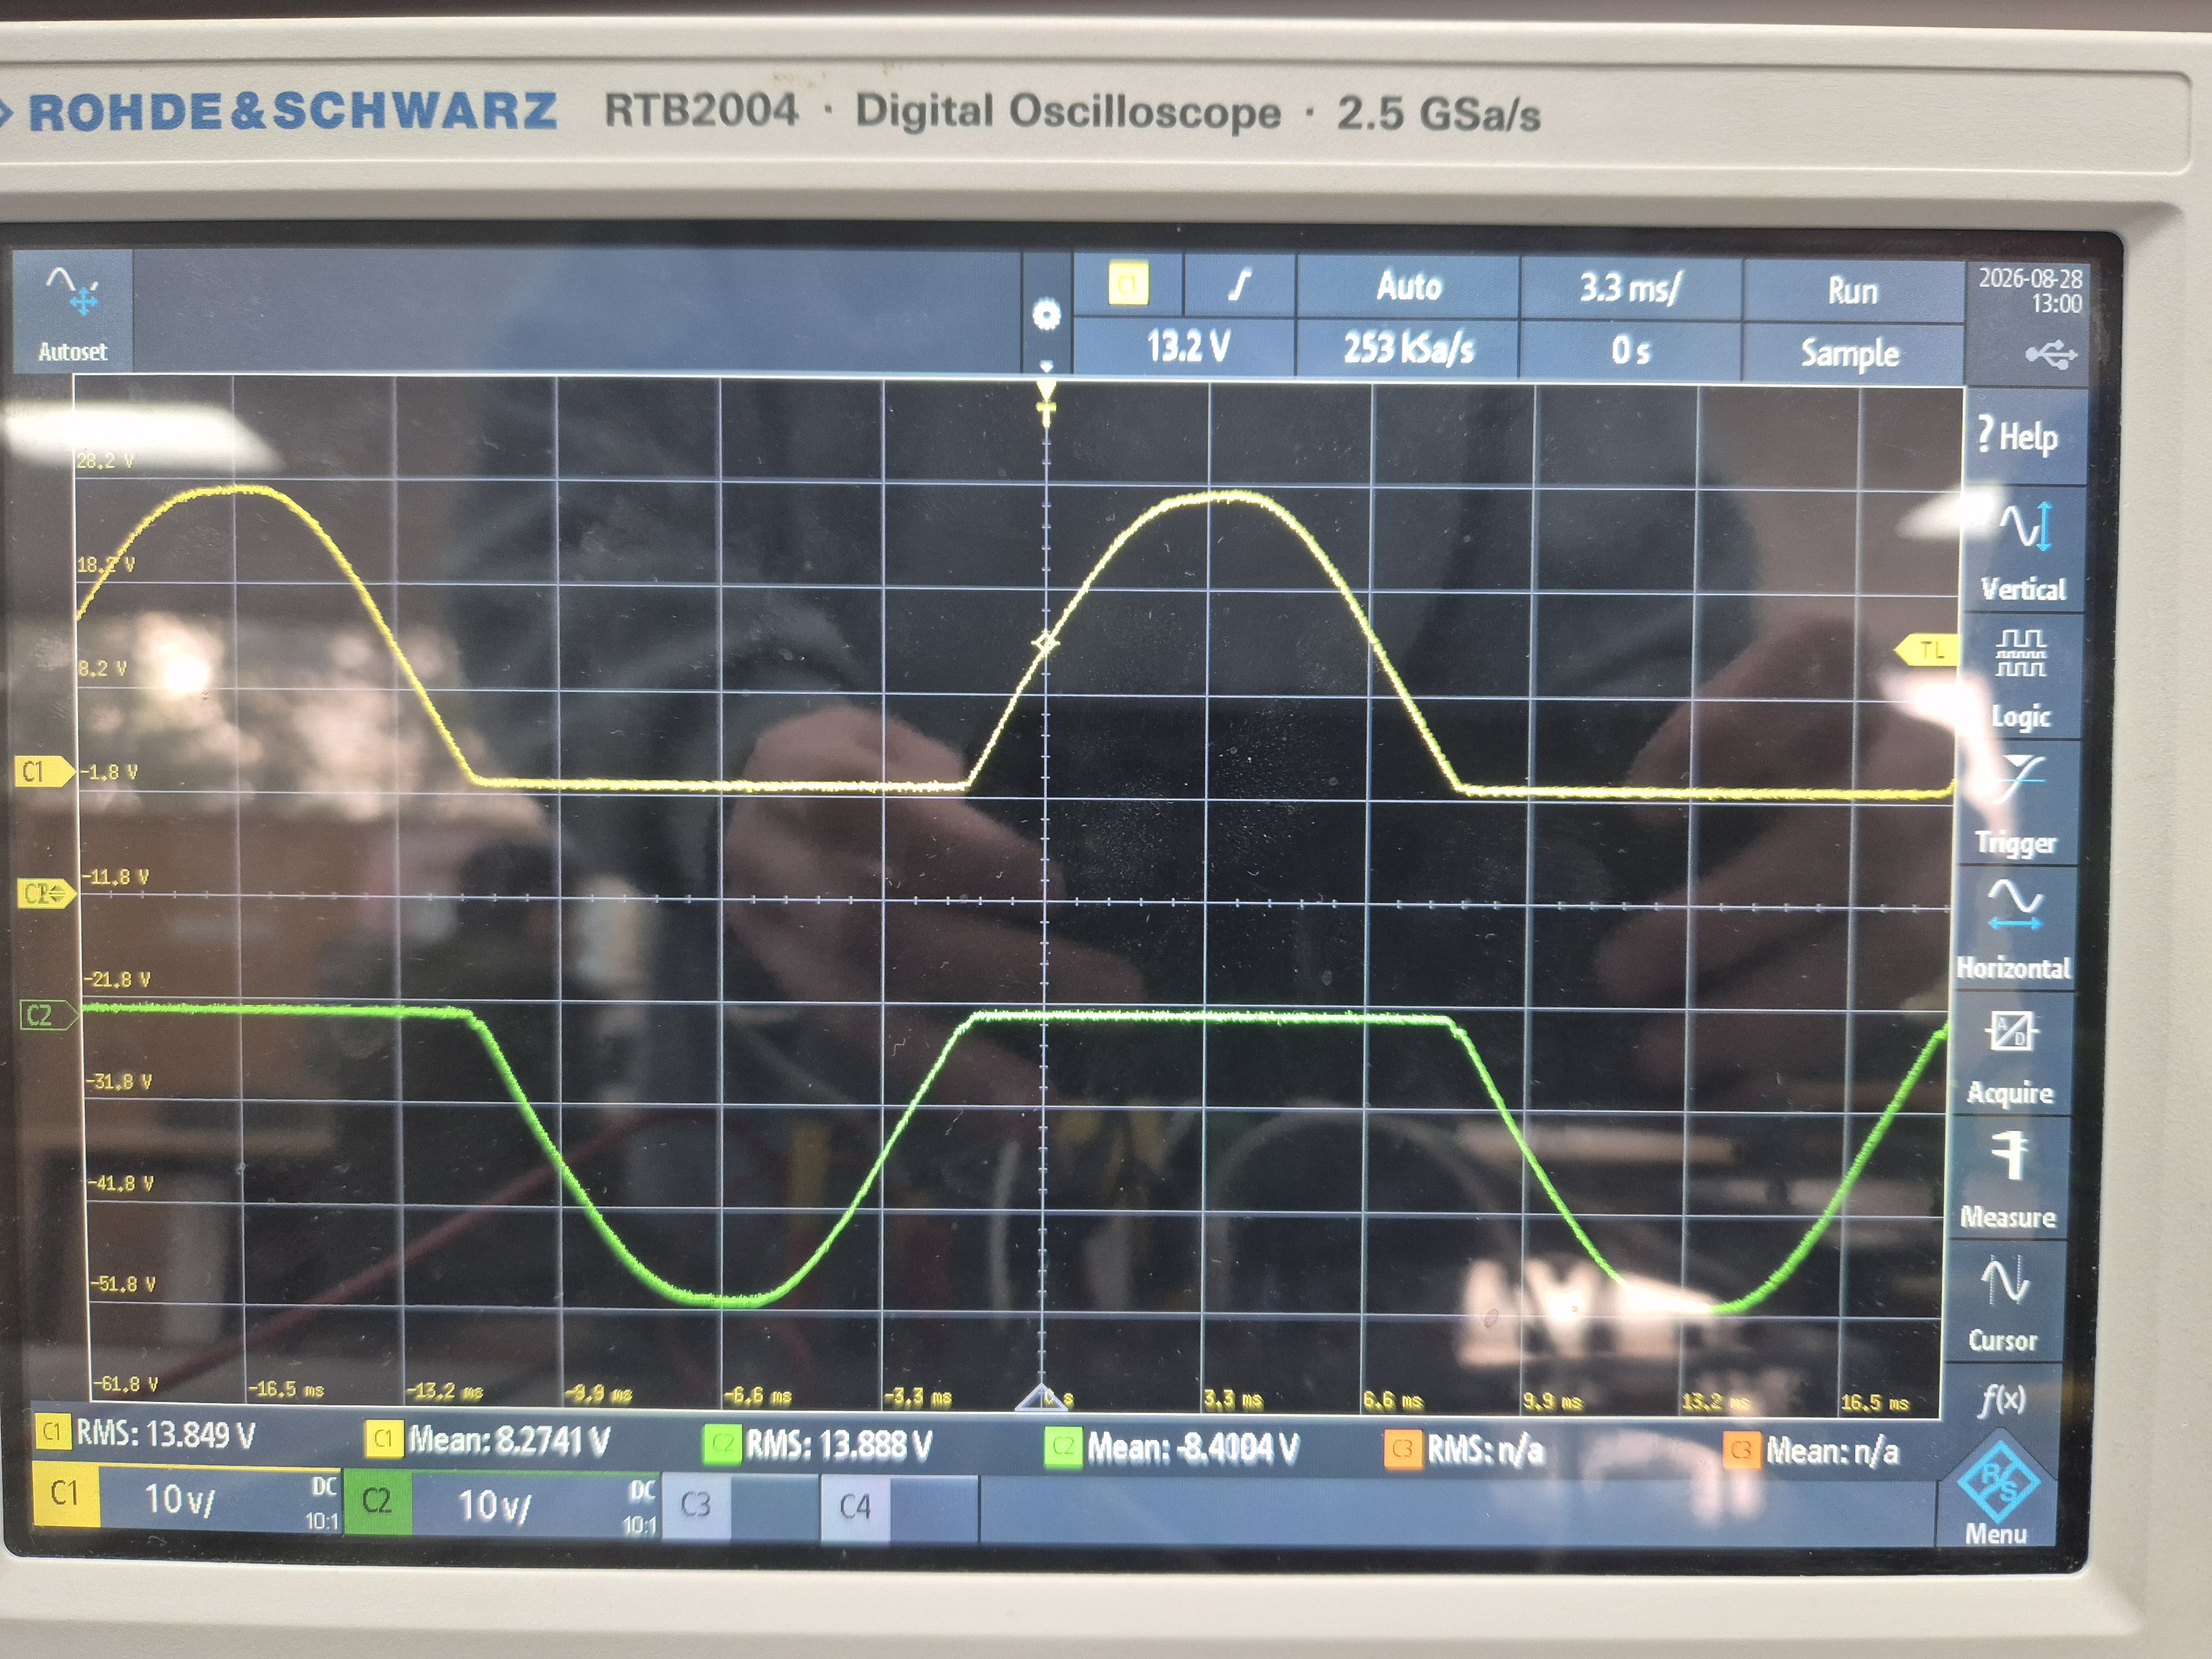
\includegraphics[width=.7\columnwidth]{Images/20250828_131136.jpg}
\caption{Voltage across diodes \(D_2\) and \(D_3\). Note: \(D_3\) is the negative voltage \label{fig:figure4}}
\end{figure}

In Figure \ref{fig:figure4} it can seen how the rectifier works. When the source voltage is positive the voltage across \(D_3\) is zero and the voltage across \(D_2\) is the source voltage. And vice versa for negative voltages, this results in a full-wave rectified voltage at the output. If the voltage across \(D_1\) and \(D_4\) were recorded we would expect that \(D_1 = D_2\) and \(D_3 = D_4\).\\

\textit{Present your measured average (dc) and rms values of output voltage and current (for RL load).
How do they compare to the values measured for the resistive load only and why?}\\

\begin{table}[H]
\caption{Measured DC and rms voltage and DC current for full-wave rectifier with resistive and inductive load \label{tab:table3}}
\centering
\begin{tabular}{|c|c|c|}
\hline
DC Voltage (V) & rms Voltage (V) & DC Current (mA)\\
\hline
11.4 & 15.1 & 332\\
\hline
\end{tabular}
\end{table}

Comparing Table \ref{tab:table2} and \ref{tab:table3} it can be seen that the DC voltage is lower, and the DC current is the same, when there is an inductor in the load. This is because the inductor stores energy when the input voltage is high and releases it when it is low, reducing the output voltage. As for the equal current, this is because the inductor has no effect on the average current, as seen by the differential equation $v = L \frac{di}{dt}$, the voltage is dependent on the change in current.\\

\textit{By considering losses in the four diodes, estimate your overall rectifier circuit efficiency. Note: there
are a few approaches you can take here, some which may require you to think about and perform
some more measurements in the lab.}\\

Diodes experience three types of losses, forward power loss \(P_F\), reverse power loss \(P_R\) and reverse recovery loss \(P_{RR}\) (\cite{DiodeEquations}). The losses are equal for each diode, so we only need to calculate the loss for one cycle and then multiply the result by four.

First lets calculate the forward losses, using data from (\cite{6A10DataSheet}) and Table \ref{tab:table3}.\\
\begin{align*}
P_F &= V_F\cdot I_F \\
P_F &= V_F\cdot \frac{I_{DC}}{2} \\
P_F &= 0.95\cdot \frac{332\cdot 10^{-3}}{2} \\
P_F &= 0.1577\ W
\end{align*}

Next lets calculate the reverse losses, using data from Table \ref{tab:table3}.
\begin{align*}
P_R &= V_R\cdot I_R \\
P_R &= \frac{V_D}{2}\cdot \frac{I_{DC}}{2} \\
P_R &= \frac{13.9}{2}\cdot \frac{332\cdot 10^{-3}}{2} \\
P_R &= 1.1537\ W
\end{align*}

Lastly the reverse recovery loss, which would be calculated using \(P_{RR} = \frac{1}{6}V_RI_{RM}t_{rr}f\), however we did not find \(I_{RM}\). Although \(P_{RR}\) would be minimal because \(t_{rr} \approx 1\ \mu s}0\) and \(I_{RM}\) would be measured in micro amps. Hence \(P_{RR}\) would have very little effect on the overall power loss of the rectifier.

Now we can calculate the efficiency of the rectifier, using data from the previous calculations and from Table \ref{tab:table3}.
\begin{align*}
P_L &= 4\cdot P_F + 4\cdot P_R \\
P_L &= 4\cdot 0.16 + 4\cdot 1.15 \\
P_L &= 5.25\ W \\
&\\
P_T &= P_L + P_{load} \\
P_T &= 5.25 + \frac{11.4^2}{48} \\
P_T &= 8.0\ W \\
&\\
\eta &= \frac{5.25}{8.0} \\
\eta &= 65\%
\end{align*}

\subsection{Full-Wave Rectifier with Capacitive Output Filter and Resistive Load}
\textit{Tabulate, to allow for easy comparison, your measured dc output voltage and peak-to-peak ripple for each of the three capacitors values}\\

\begin{center}
	\begin{tabular}{|c|c|c|}
		\hline
		\centering\textbf{Capacitor Size} & \centering\textbf{DC Output Voltage $V_{dc}$} &\centering\textbf{Peak-to-Peak Ripple $V_{pp}$}\tabularnewline 
		\hline
		$470 F$ & $2.1V$ & $7V$ \\
		\hline
		$1000 F$ & $1.2V$ & $4.4V$\\
		\hline
		$2000 F$ & $0.5V$ & $2.35V$\\
		\hline
	\end{tabular}
\end{center}

\textit{Carefully plot (using data saved from the oscilloscope) or sketch by hand on one graph the output voltage waveform observed for each of the three capacitor values. Comment on how and why the
waveforms and measurements differ with changing capacitor value.}\\

These plots show how the capacitive output filter effects the output voltage and current waveforms. As the capacitor size increases the smoothing effect also increases. This is because the time for the capacitor to charge and discharge also changes. As the AC input increases the capacitor charges, then as the input is negative the capacitor discharges. The time constant $\tau=R_LC$ effects the charging time of the capacitor, appearing in the plots as more ripple in the output voltage with the smaller capacitor values.\\
\begin{figure}[H]
        \centering
	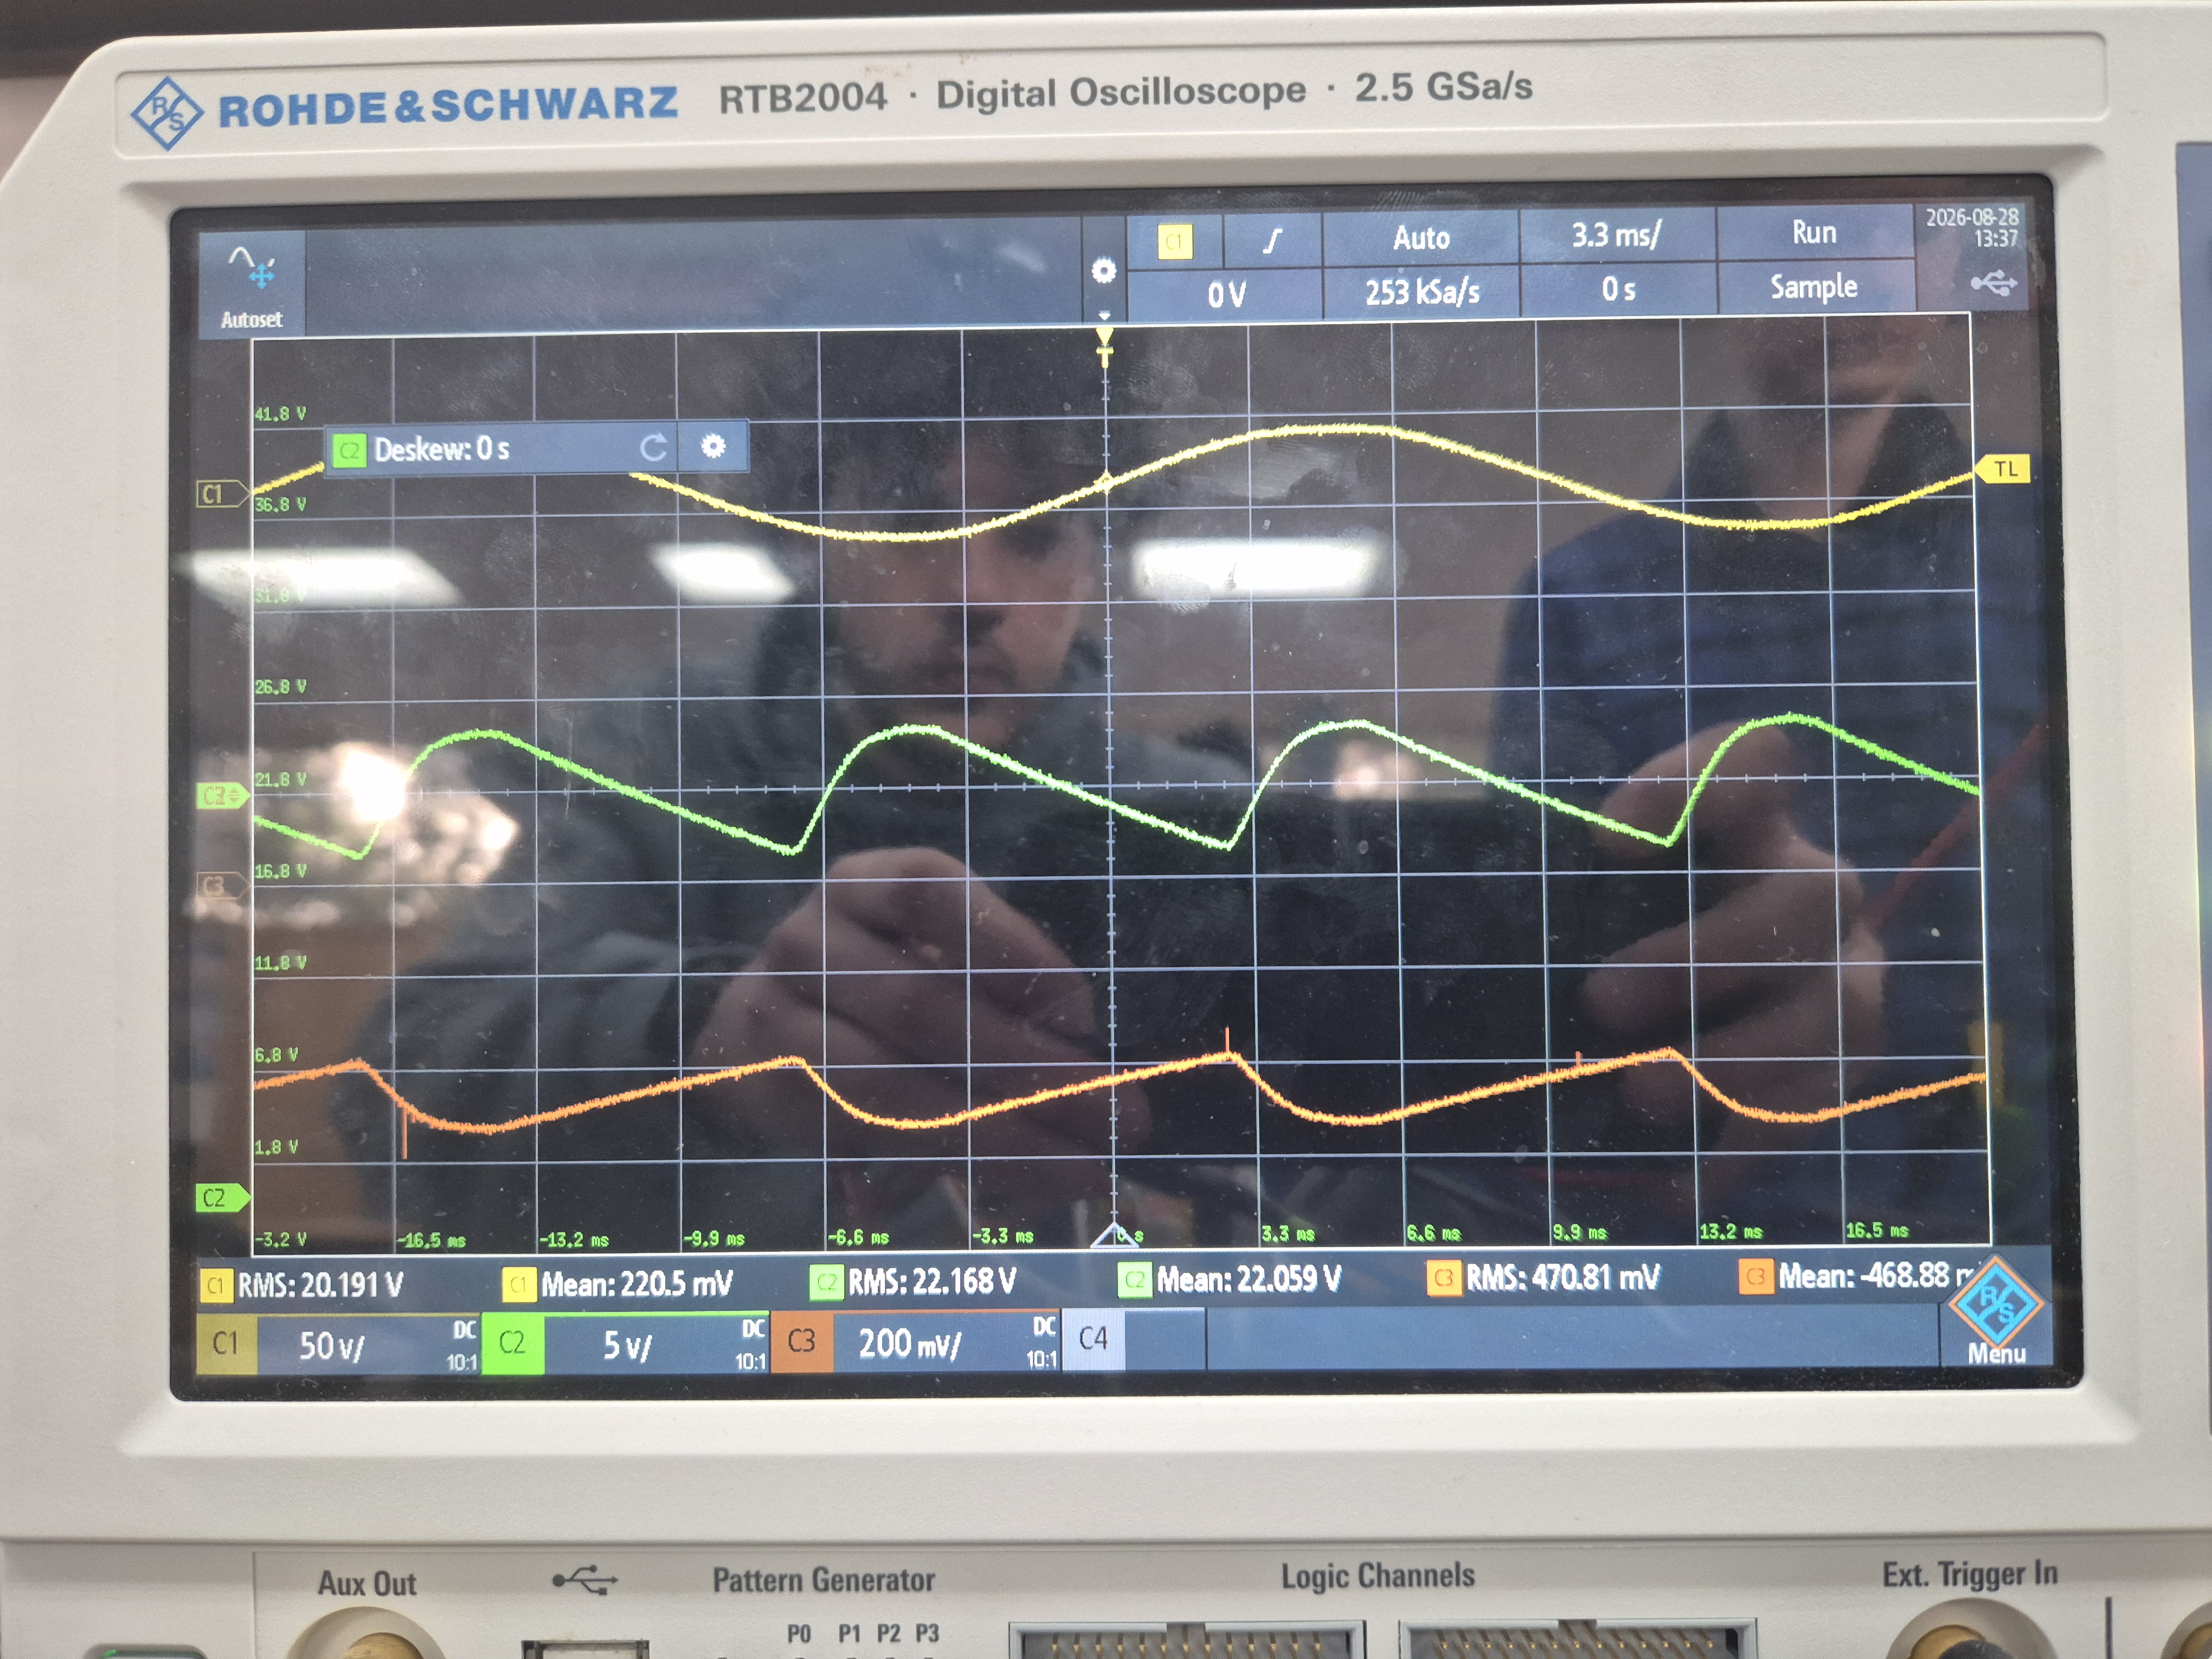
\includegraphics[width=0.7\columnwidth]{Images/20250828_134829.jpg}
	\caption{$470\:\mu F$ Capacitor Plot}
	\label{fig:470F Cap Plot}
\end{figure}
\begin{figure}[H]
        \centering
	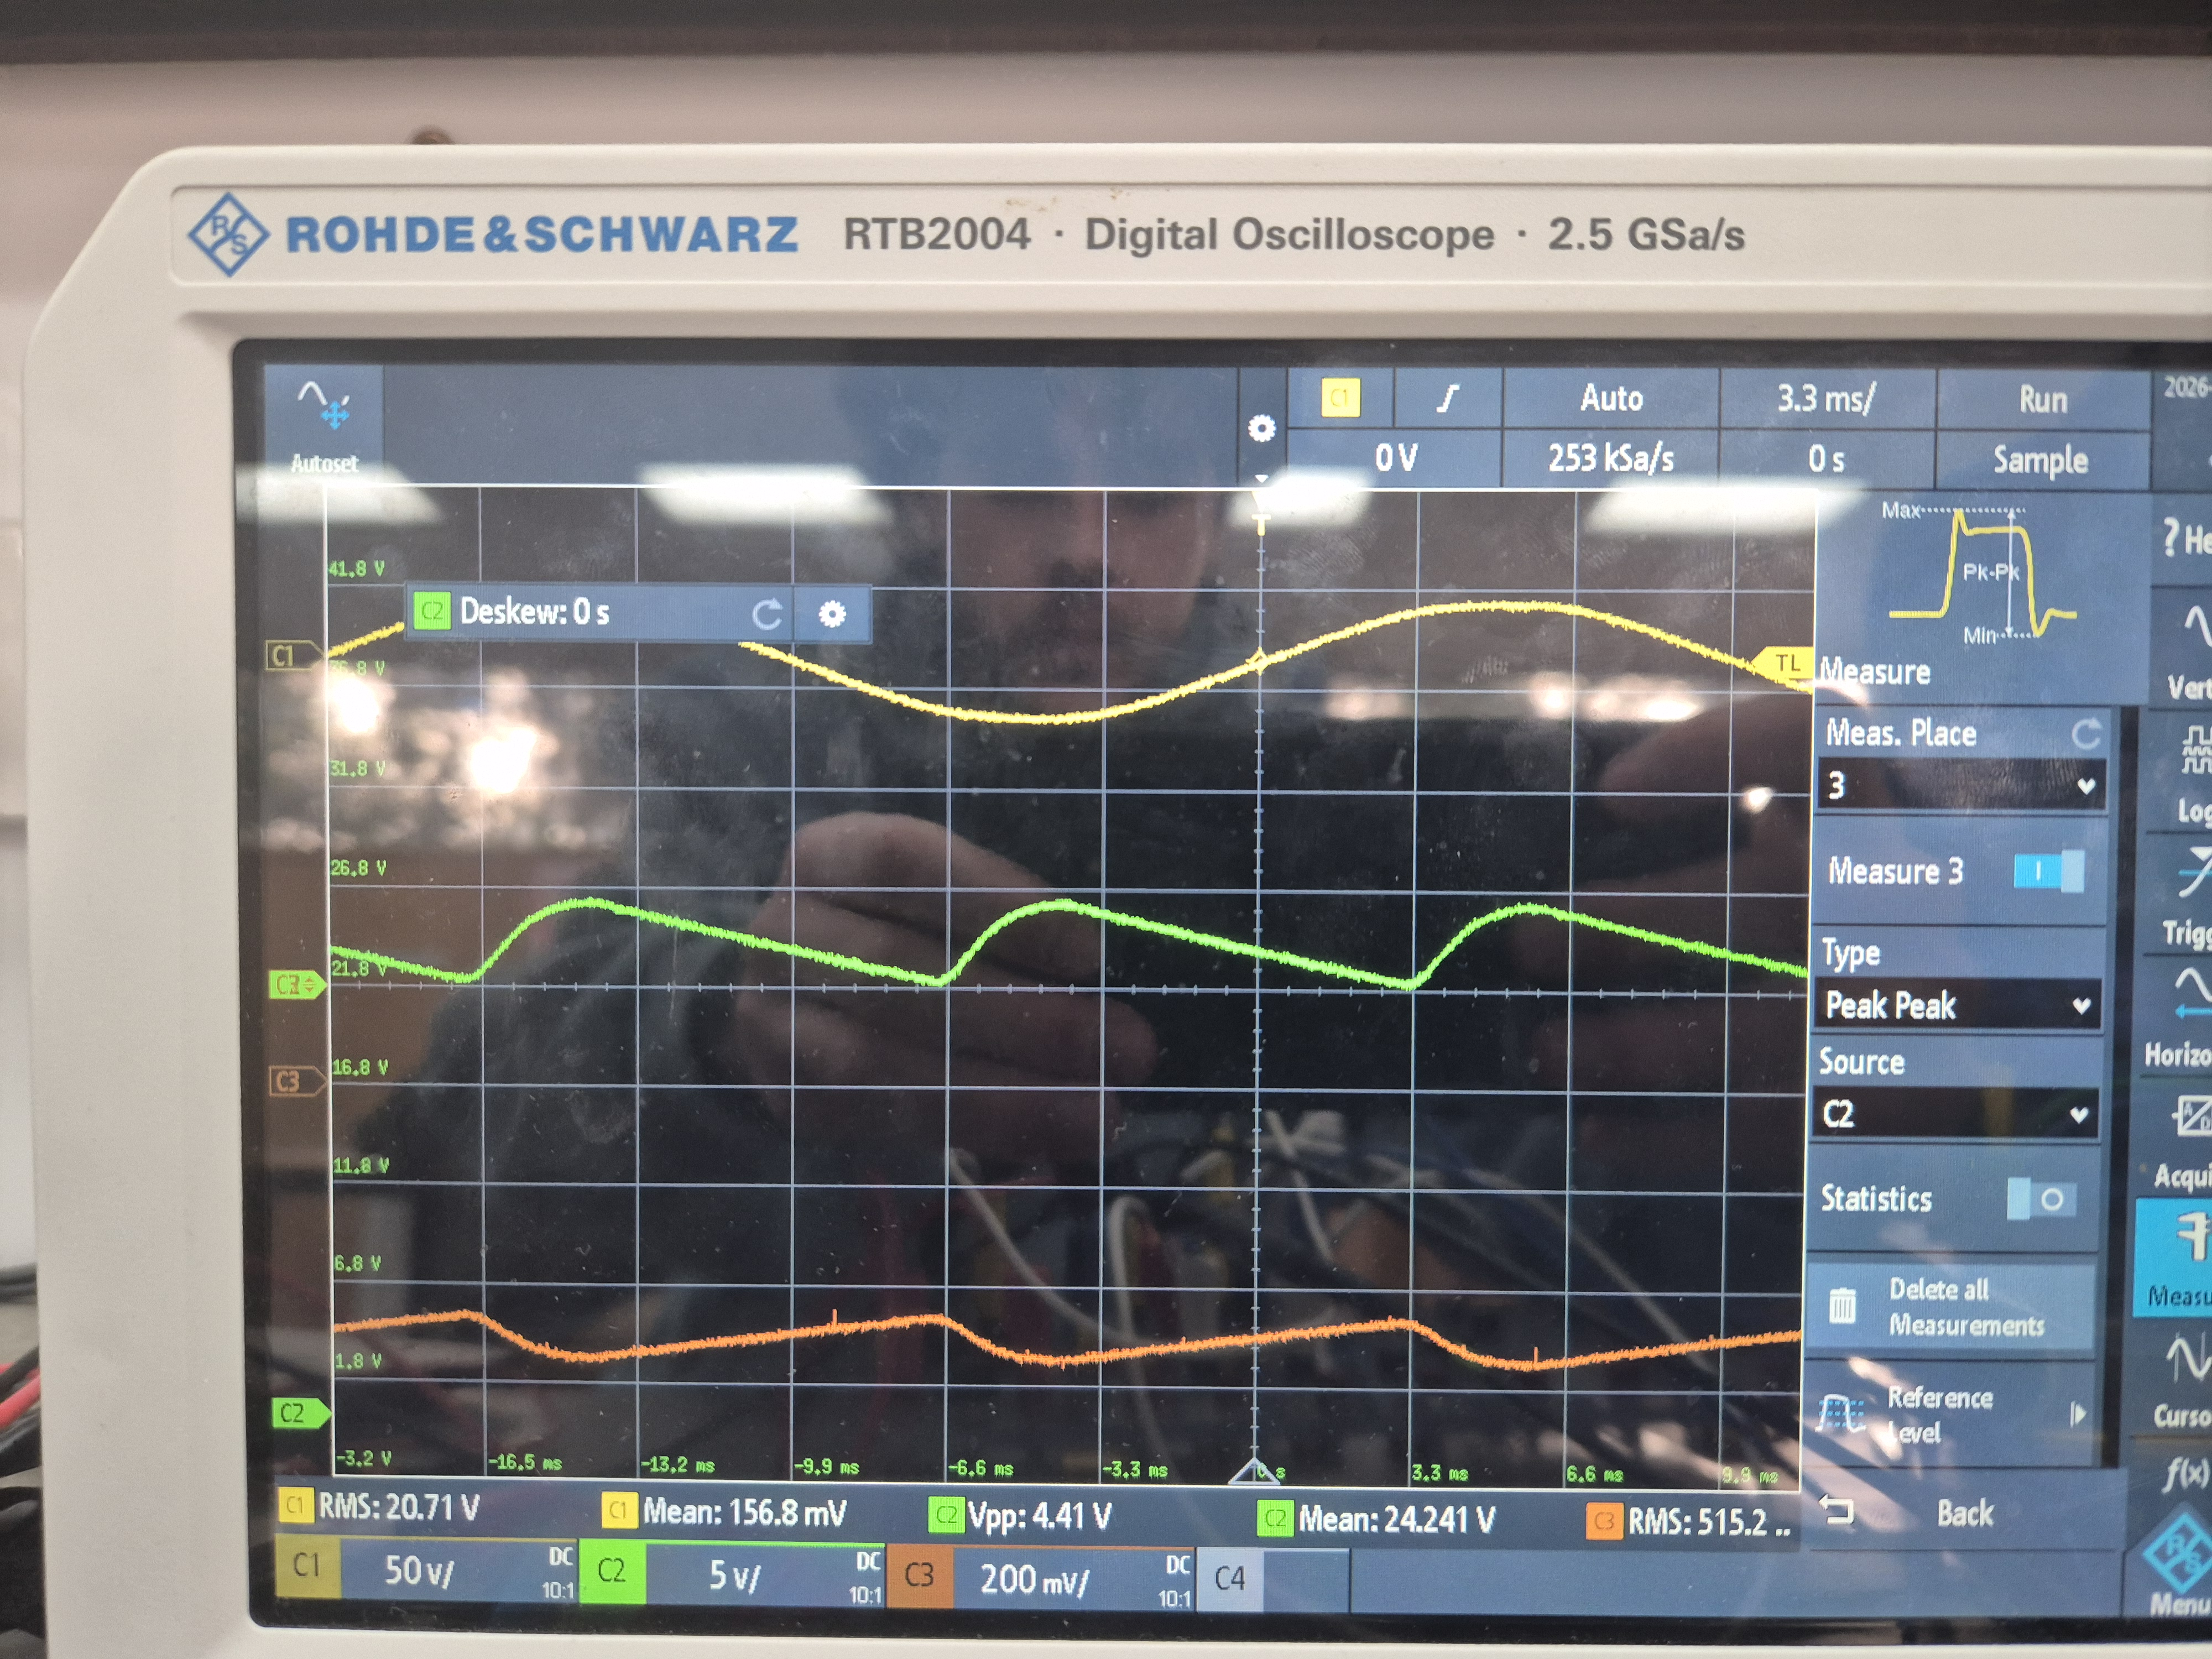
\includegraphics[width=0.7\columnwidth]{Images/20250828_135102.jpg}
	\caption{$1000\:\mu F$ Capacitor Plot}
	\label{fig:1000F Cap Plot}
\end{figure}
\begin{figure}[H]
        \centering
	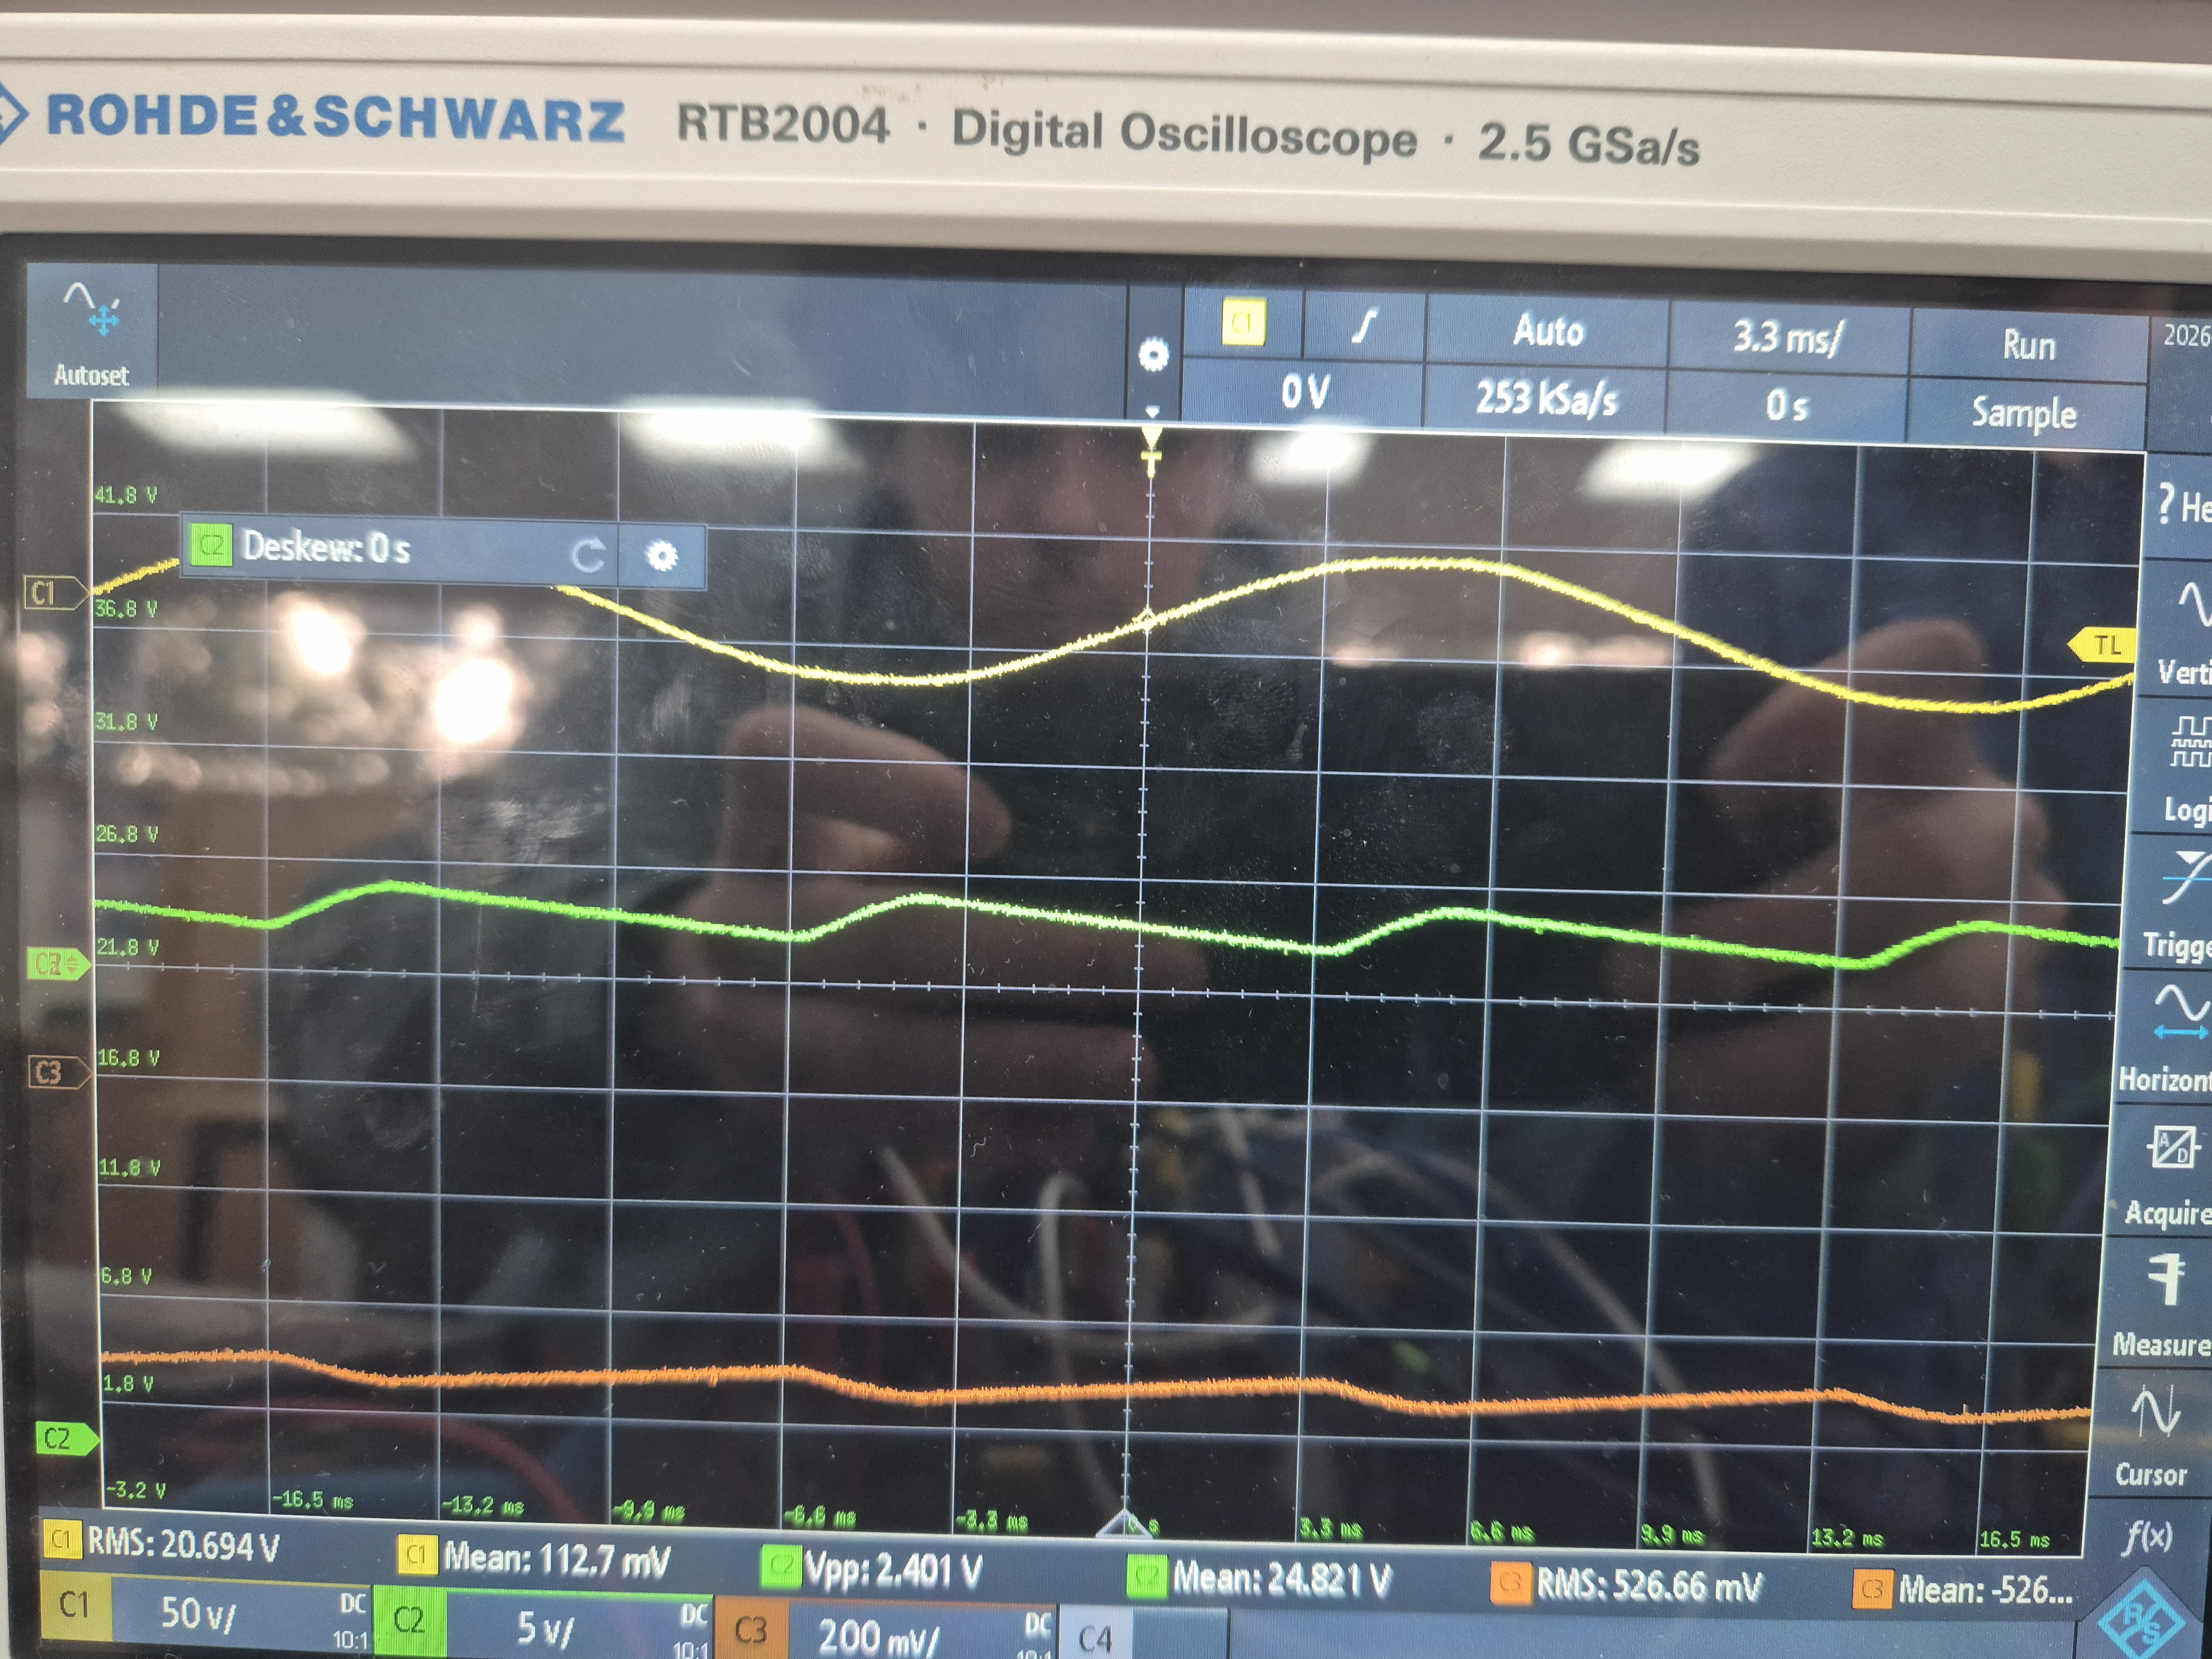
\includegraphics[width=0.7\columnwidth]{Images/20250828_135318.jpg}
	\caption{$2000\:\mu F$ Capacitor Plot}
	\label{fig:2000F Cap Plot}
\end{figure}


\textit{Develop an approximate expression for percentage peak-to-peak ripple as a function of R, C and frequency $f$, stating carefully any assumptions. How do your calculated values, using your derived expression, compare to your measurements?}\\

Using the capacitor discharge over on ripple period the percentage peak-to-peak ripple can be calculated.
$$\Delta\approx\dfrac{V_{DC}}{R_LC}\cdot\dfrac{1}{2f}$$
$$r_{pp}(\%)\approx\dfrac{100}{2fR_LC}$$
Comparing this to the measured results with the $1000\:\mu F$ capacitor.
$$r_{pp,calc}(\%)\approx\dfrac{100}{2*50*48*1000*10^{-6}}=20.83\%$$
$$r_{pp,measured}(\%)\approx18.2\%$$
This expression is a good approximation to the peak-to-peak ripple measured on the plot.\\

\textit{How would you expect the value of the capacitor to impact upon supply current waveform, in particular on the harmonic content? Describe why you expect this? (Note: if you have time you may wish to think of a way to measure and display the Fourier components of supply current for your circuit, thus gaining extra insight}\\

Increasing the capacitance makes the rectifier's output ripple smaller, but it also makes the supply current more impulsive. As the capacitor size increases the Total Harmonic Distortion also increase. This leads to the distortion power factor deteriorating, also worsening the overall power factor. This also means there are more harmonics. The harmonic currents only affect the RMS current without increasing the real power so the power factor decreases.\\ 

\section{Thyristor Controller Rectifiers}
\subsection{Semi-Converter with Resistive and Inductive Load}
\begin{center}
\begin{tabular}{|p{3cm}|p{2.5cm}|p{2.5cm}|p{2.5cm}|}
\hline
\centering\textbf{Firing angle} &
\multicolumn{2}{c|}{\textbf{Digital multimeter}} &
\centering\textbf{Calculated} \tabularnewline
\hline
\centering$\alpha$ & \centering$V_o(V)$ & \centering$I_o(mA)$ & \centering$V_o(V)$ \tabularnewline
\hline
0 & 0 & 0 & 0 \\ \hline
20 & 0.8 & 0.8 & 0.384 \\ \hline
45 & 3.4 & 20 & 1.865 \\ \hline
60 & 5.6 & 63 & 3.183 \\ \hline
90 & 9.7 & 159 & 6.366 \\ \hline
100 & 10.2 & 184 & 7.471 \\ \hline
120 & 10.9 & 247 & 9.549 \\ \hline
140 & 10.6 & 285 & 11.243 \\ \hline
160 & 9.5 & 317 & 12.348 \\ \hline
180 & 8.8 & 333 & 12.732 \\ \hline
\end{tabular}
\end{center}\\
To calculate $V_o$ use the formula,
$$V_{o,theory}=K(1-cos(\alpha))$$
where,\\
$$K=\dfrac{V_m}{\pi}=6.366V$$\\
These results can be seen in the table above.\\

\textit{Detail the way you connected your oscilloscope probes and configured the oscilloscope to record simultaneously the source voltage, trigger signal, output voltage and current waveforms.}\\

The common ground is at $+V_o$ to allow for common measurements. Channel 1 measures the source voltage using the secondary transformer winding. This is acceptable as it is electrically isolated from the remainder of the circuit so multiple grounds cannot cause a short circuit. Channel 2 measure the output voltage, with it's positive probe placed at $-V_o$. Channel 3 measures $I_o$, with it's probe placed between the $1\Omega$ and $47\Omega$ resistors. Measuring the voltage over the $1\Omega$ resistor is equivalent to measuring current as $V=IR$. Channel 4 measures the positive trigger input of $T_1$. \\ 

\textit{Include plot from oscilloscope of all waveforms for a firing angle of 45°.}\\

Channel 2 and Channel 3 show the negative output voltage and output current respectively as their ground and positive connections are inverted due to needing a common ground point for all measurements. 
\begin{figure}[H]
        \centering
	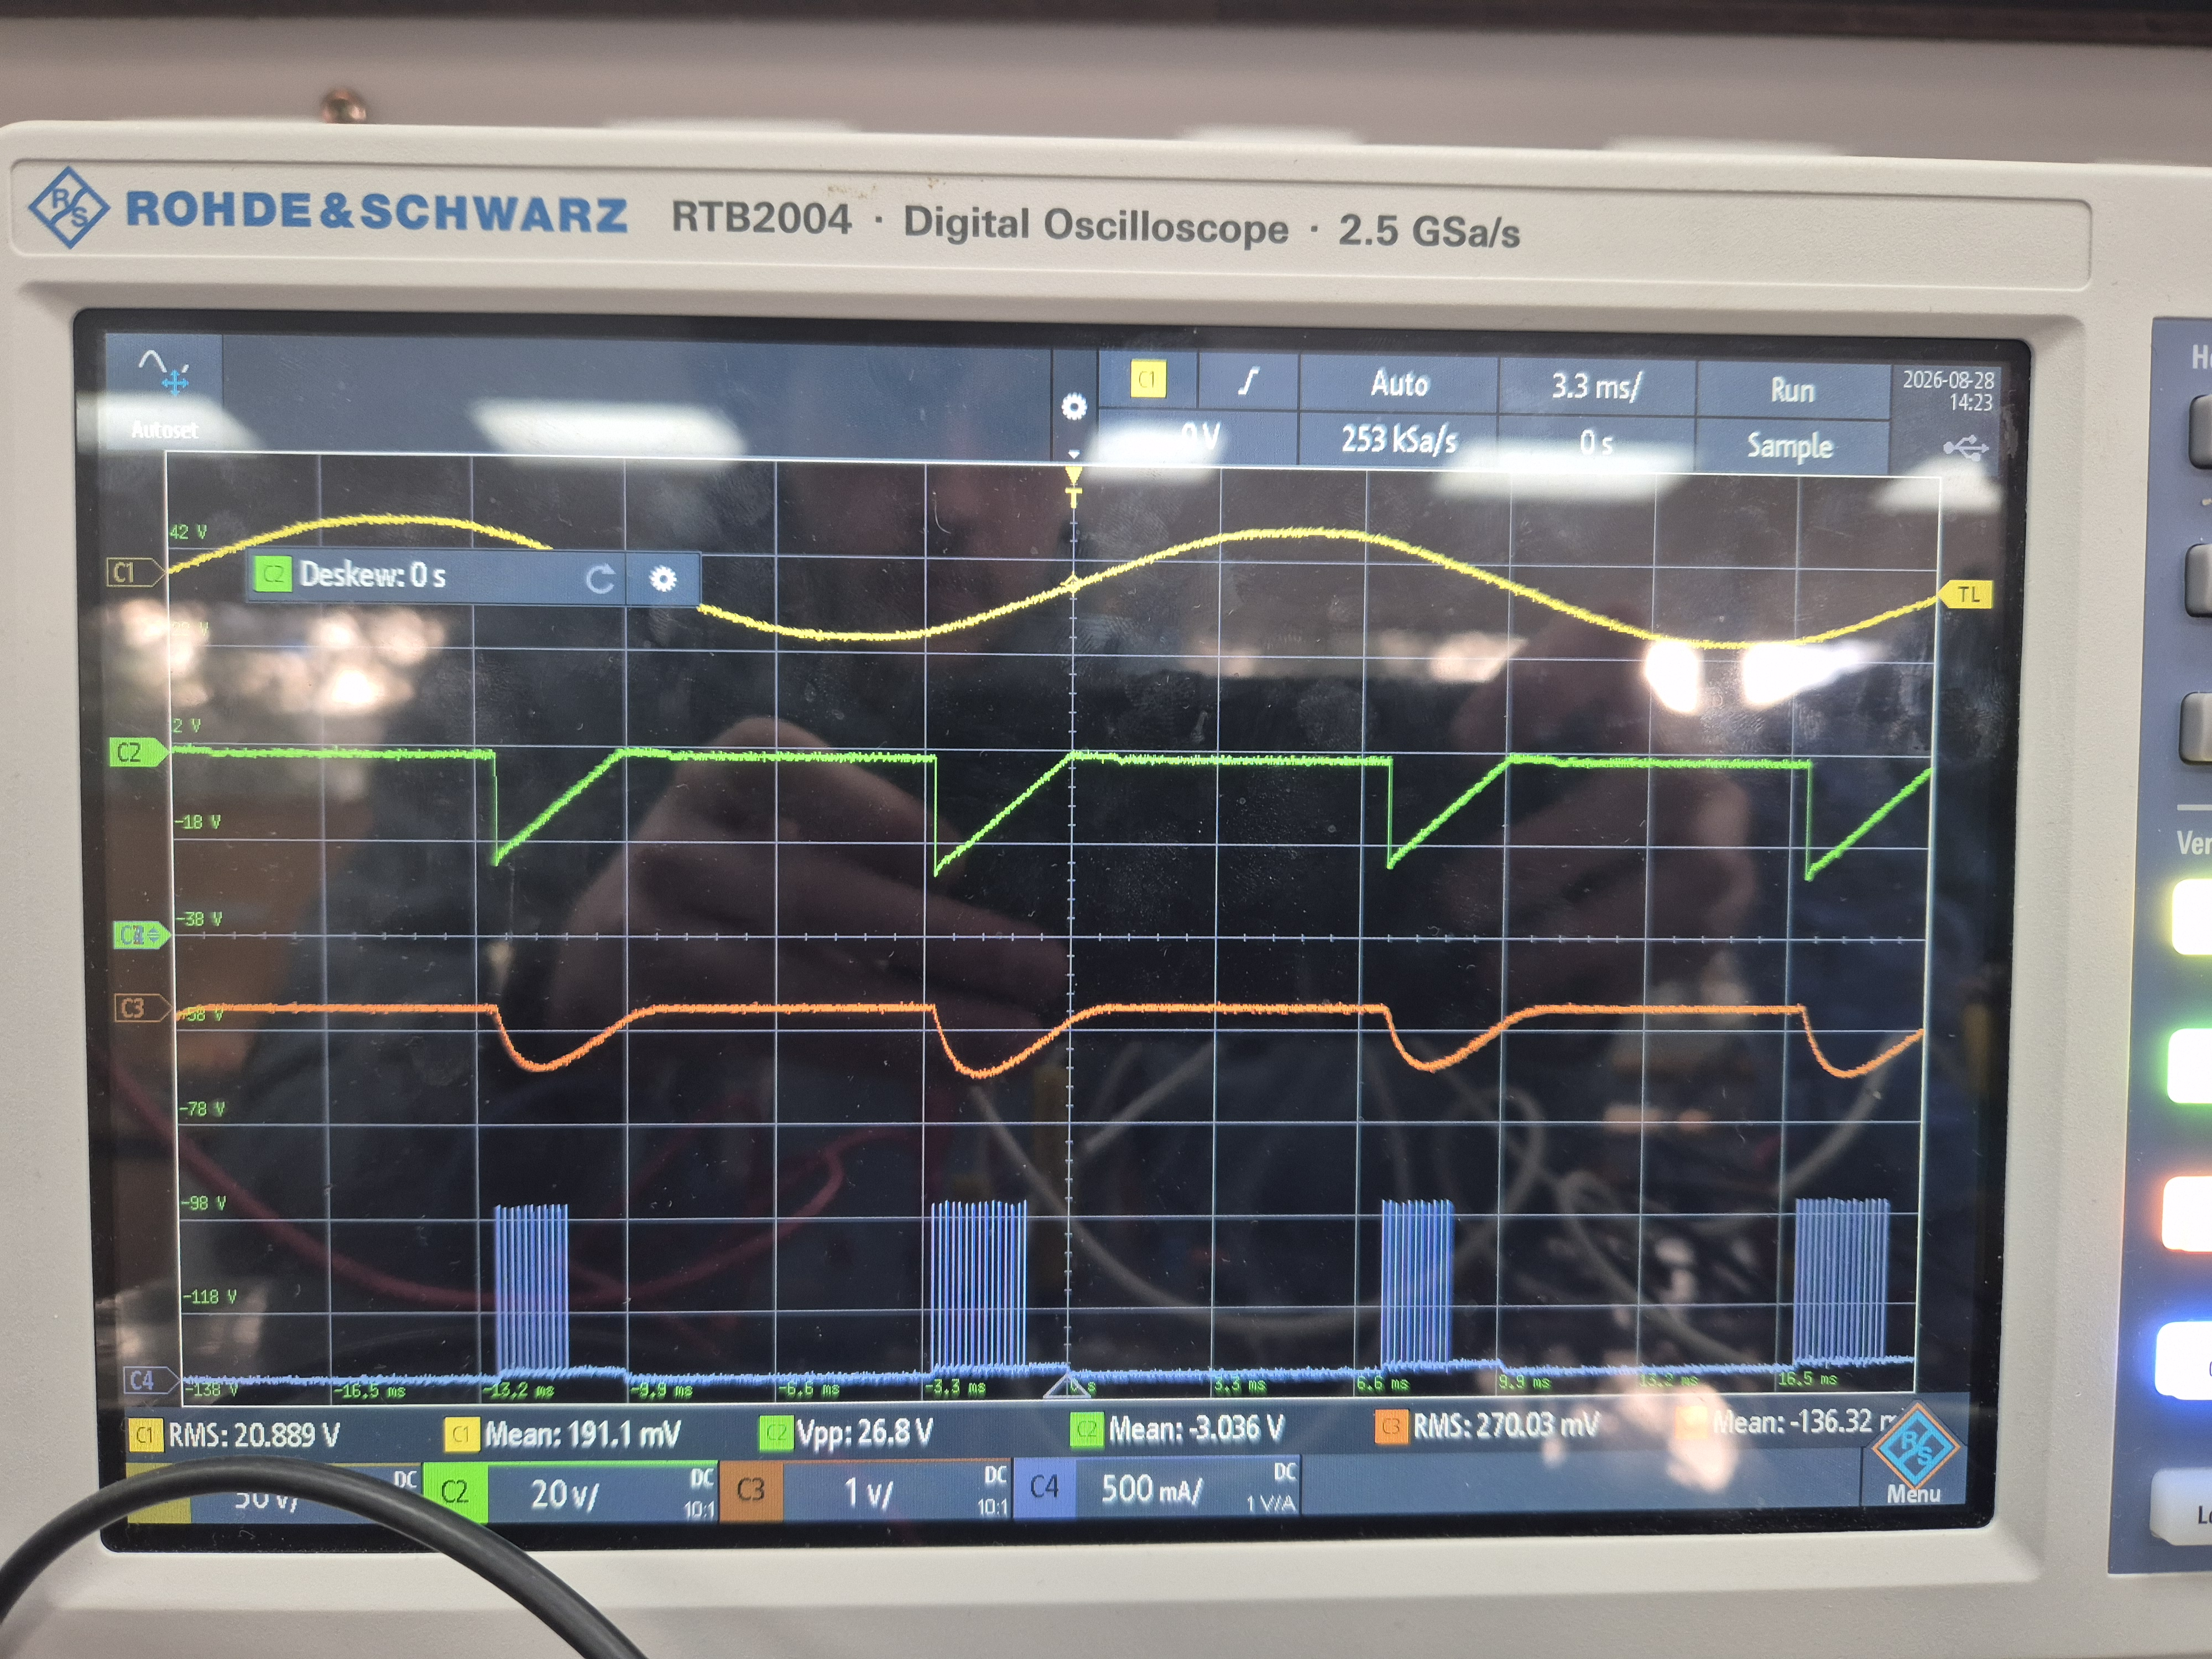
\includegraphics[width=0.7\columnwidth]{Images/20250828_143455.jpg}
	\caption{$45\degree$ firing angle}
	\label{fig:45 degree firing angle}
\end{figure}

\textit{Comment on the observed waveforms and on how they changed with firing angle, describing your observations by considering theory of the circuit operation.}\\

As the firing angle is increased to $180\degree$ the output voltage and current approach the full wave rectified input waveform shown by Channel 1. This is beaus at a firing angle of $180\degree$ the thyristor acts the same as a typical diode used in a full wave rectifier.\\

\textit{From your measured data, create a plot of DC output voltage vs firing angle. Also include in the plot a curve based on theoretical considerations for this circuit. Discuss your findings.}\\

\begin{figure}[H]
        \centering
	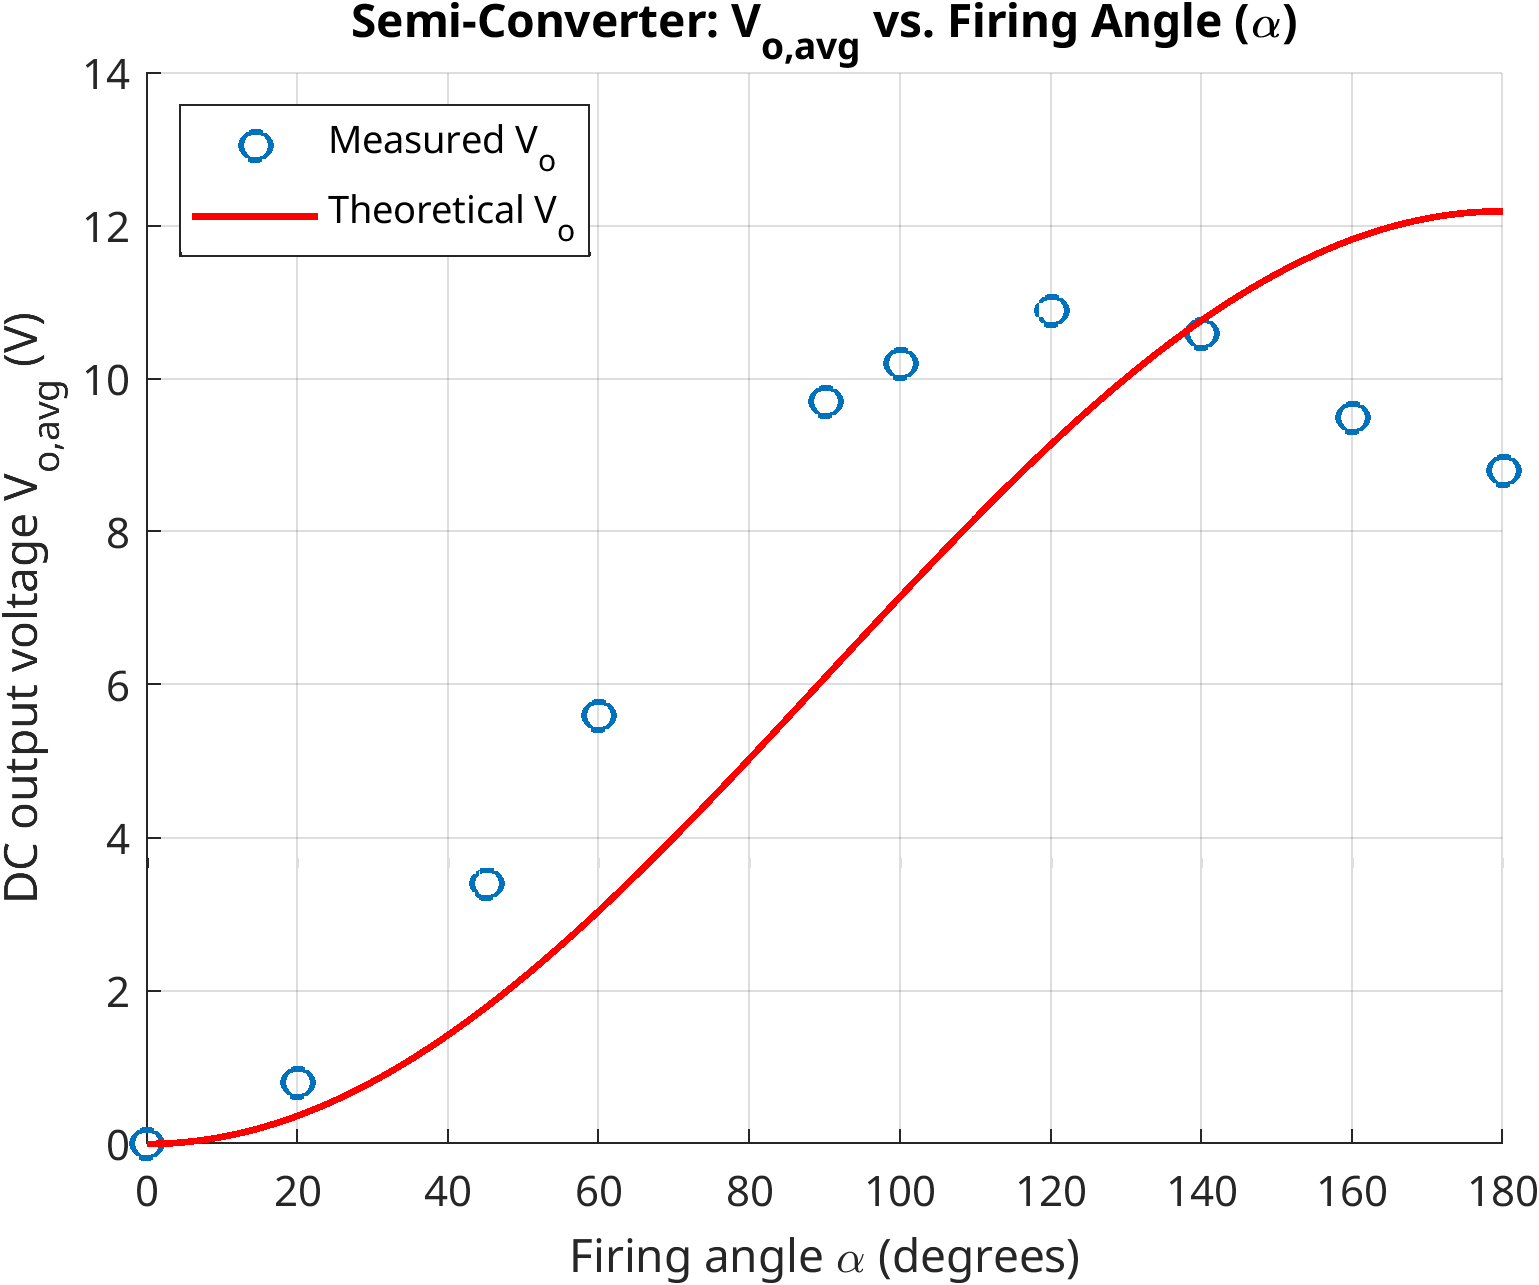
\includegraphics[width=0.7\columnwidth]{Images/semi_converter_correct.png}
	\caption{Output Voltage vs Firing Angle}
	\label{fig:output voltage vs firing angle}
\end{figure}

The theoretical curve $V_{dc}=K(1-\mathrm{cos}\:\alpha)$ matches the measured results with an acceptable error. At a small firing angle the deviations are caused by discontinuous current. The error at higher firing angles may be attributed to residual conduction in the load. There may also be isomer error caused by the non-idealities in the lab configurations.\\

\textit{Based on your observation, at what firing angle did you observe there to first be a boundary between continuous and discontinuous conduction (of current in the load). Compare to what you might expect from a theoretical view point?}\\

The data suggests that the rectifier is is discontinuous conduction mode until approximately $50\degree$ as the average output current is very low suggesting the current drops to zero for parts of the cycle. Above $60\degree$ the output current increases significantly as $\alpha$ increases confirming the current is in continuous conduction mode.\\
Theoretically current should be continuous as long as long as the firing time is long enough for the inductor to store energy to prevent zero current between firing pulses. This means that discontinuous current is expected for low values of $\alpha$ as seen through the measurements.\\

\textit{Describe the purpose of the freewheeling diode in this circuit and what you think might happen if it were removed.}\\

The freewheeling diode provided a safe path for current to flow when the AC input voltage reverse polarity or if the thyristors are turned off. The inductor inherently opposes and sudden current change so a path is required to allow for a gradual decay. This prevents damage to components due to large voltage spikes across the thyristors. It also improves the rectifiers performance by reducing output voltage ripple and smoothing the load current.\\
If the freewheeling diode where to be removed the inductor current would have no alternate discharge paths, leading to discontinuous conduction, higher output ripple and potentially cause damage to the thyristors due to the inductor's stored energy.

\section{Reflection}

TODO: 
\newpage

\printbibliography

\vfill
\hrule
\begin{center}
\textit{End of Report}
\end{center}
\end{document}
